\lab{Algorithm}{Line Sweep}{Line Sweep}

\objective{Learn about and implement a basic line sweep algorithm}

\section*{General Line Sweep Algorithms}

Line sweep algorithms are a significant group of algorithms with a variety of applications. 
In the strictest sense, line sweep algorithms typically use a priority queue and binary tree to lower the temporal complexity associated with certain tasks. 
Some notable examples include Fortune's Algorithm for calculating Voronoi diagrams and Andrew's Algorithm for computing the convex hull of a set of points. 
In this lab, we will explore a basic line sweep algorithm that allows efficient computation of the Closest Pair problem.  
Given a set of points, find the distance between the closest pair of points.

\section*{Na\"ive Implementation}

The obvious way of doing this is to simply compute the distance between each point and each of the other points.
Roughly speaking, this requires some constant multiple of $n^2$ computations where $n$ is the number of points.
This can be coded as follows:
\begin{lstlisting}
def reallybadmindist(X):
    r = ((X[0]-X[1])**2).sum()**.5
    for i in range(len(X)):
        for j in range(len(X)):
            if i != j:
                r = min(r,((X[i]-X[j])**2).sum()**.5)
    return r
\end{lstlisting}
Since distance is symmetrical, we can compare each point with the points that follow it in the list we are given (which will reduce
the total number of distances to be computed).
This is a sleightly better implementation:
\begin{lstlisting}
def multidist(p0,p1):
    l=len(p0)
    return sum([(p0[i]-p1[i])**2 for i in range(l)])**.5
def badmindist(X):
    l=len(X)
    r=multidist(X[0],X[1])
    for i in xrange(l):
        for j in xrange(i+1,l):
            d=multidist(X[i],X[j])
            if d<r:
                r=d
    return r
\end{lstlisting}

Since,on average, we iterate through about half of the list for each point added, this algorithm will have complexity $O(n^2)$ (we are only scaling by a constant factor).  
It is faster than the truly na\"ive method, but essentially just as inefficient.
For very small numbers of points, this algorithm works, but it quickly becomes inefficient as we increase the number of points processed.  
What we would like to do is go from $O(n^2)$ to something better.  
To do this, we have to think about the problem differently.
This can be done by using one of the key techniques of computational geometry-a line sweep algorithm.

\section*{A Simplified Line Sweep Algorithm}

The concept behind a line sweep algorithm is breaking a global problem into a sequence of smaller problems that can be solved locally.
We sweep the domain space with a line.
This line divides the domain space into an explored region and an unexplored region.
As the line sweeps, events occur, be it whether the line encounters a point in the data set
or some other type of event.  
We compute the solution at the very beginning of the line sweep and as new events happen, we compute the change that these events have on our current solution.
We only need to consider the events in the explored region or on the sweep line as they are the only events that affect the current solution.  
Sweep line algorithms typically exhibit a temporal complexity of $O(n \log n)$, which is far better than $O(n^2)$.

Line sweep algorithms are good for doing all sorts of proximity based computations.
In the example above, we took advantage of the fact that distance was symmetric ($d(a,b)=d(b,a)$).
In a line sweep version of this algorithm, we also take advantage of the fact that any points further than the current smallest minimum distance along a given axis do not need to be considered.
This is really just an aplication of the triangle inequality.
The secret to the line sweep solution for the closest pair problem is to actually have two sweep lines with a small distance between them.
As we process the points in our list, we can decrease the distance between the lines so that we only process points that could possibly give a smaller distance than the smallest distance we have already encountered.
By only processing the points between our two sweep lines, we avoid processing many points needlessly.

For a general line sweep algorithm, it is common to use a priority queue to order the items that need to be processed.
A good priority queue can be found in the library \li{Queue} that is included in Python. 
In this case all we need to do is sort the points by $X$ value.
This means it will be easier to make a sorted copy of the array using numpy's built in functions.
Something like \li{X=Y.take(Y[:,0].argsort(),axis=0)} or \li{Y[Y[:,0].argsort()]} will do this for you. 

We track the points in the area between the two sweep lines with a list.
Each time we advance the sweep lines, we update this list so it always contains the points between the sweep lines (adding or removing points where necessary).
A point stays in the list if its distance from the leading sweep line is less than the current minimum distance.
Conceptually, this is how we place the second sweep line.

Assuming we have already ordered all our points by $x$ coordinate, we can perform the line sweep algorithm as follows:

\vspace{5mm}
\begin{compactenum}[1.]
\item 
Process the first two points and add them to the active list.
Set current minimum distance to the distance between these two points.
\item 
Get the next point in the priority queue.
\item 
Update the active list so that it contains only the points between the two sweep lines.
\item 
Compute the distance between the current point and all the points in the active list.
\item 
Compare the smallest distance found with the current minimum distance. 
Change the current minimum distance if needed.
\item 
Repeat steps 2 to 5 for all remaining points in the priority queue
\end{compactenum}
\vspace{5mm}

When the algorithm ends, the current minimum distance will be the distance between the closest pair of points.

This algorithm can be illustrated as follows:
\begin{figure}[H]
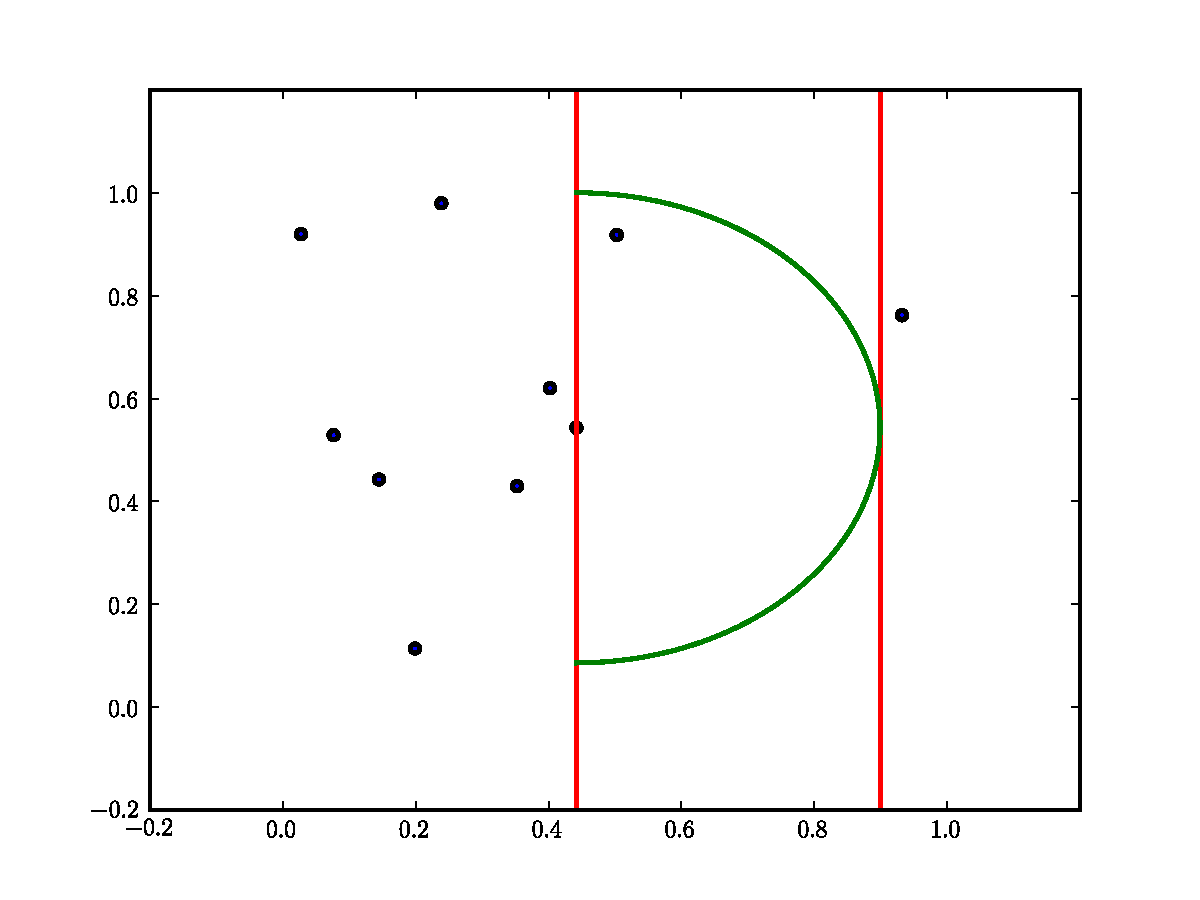
\includegraphics[width = \textwidth]{simple0.pdf}
\caption{After processing the first two points, we process the third point and change the current minimum distance accordingly.}
\end{figure}

\begin{figure}[H]
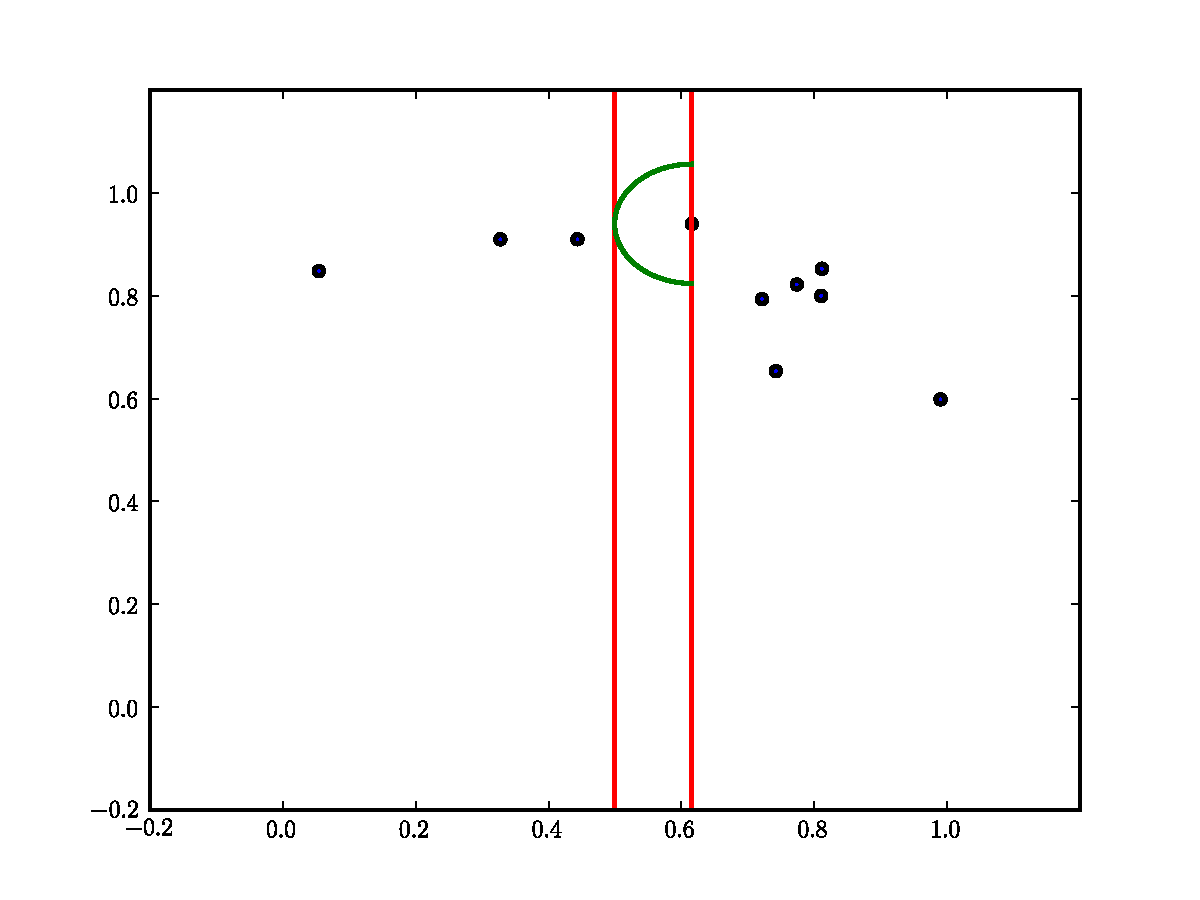
\includegraphics[width = \textwidth]{simple1.pdf}
\caption{This change in the minimum thus far is reflected in how we form the actives list for the next point we process. 
We remove the points from the top of the queue that are too far away in the $x$ direction to have a distance less than the current minimum. 
We then process anything that is left.}
\end{figure}

\begin{figure}[H]
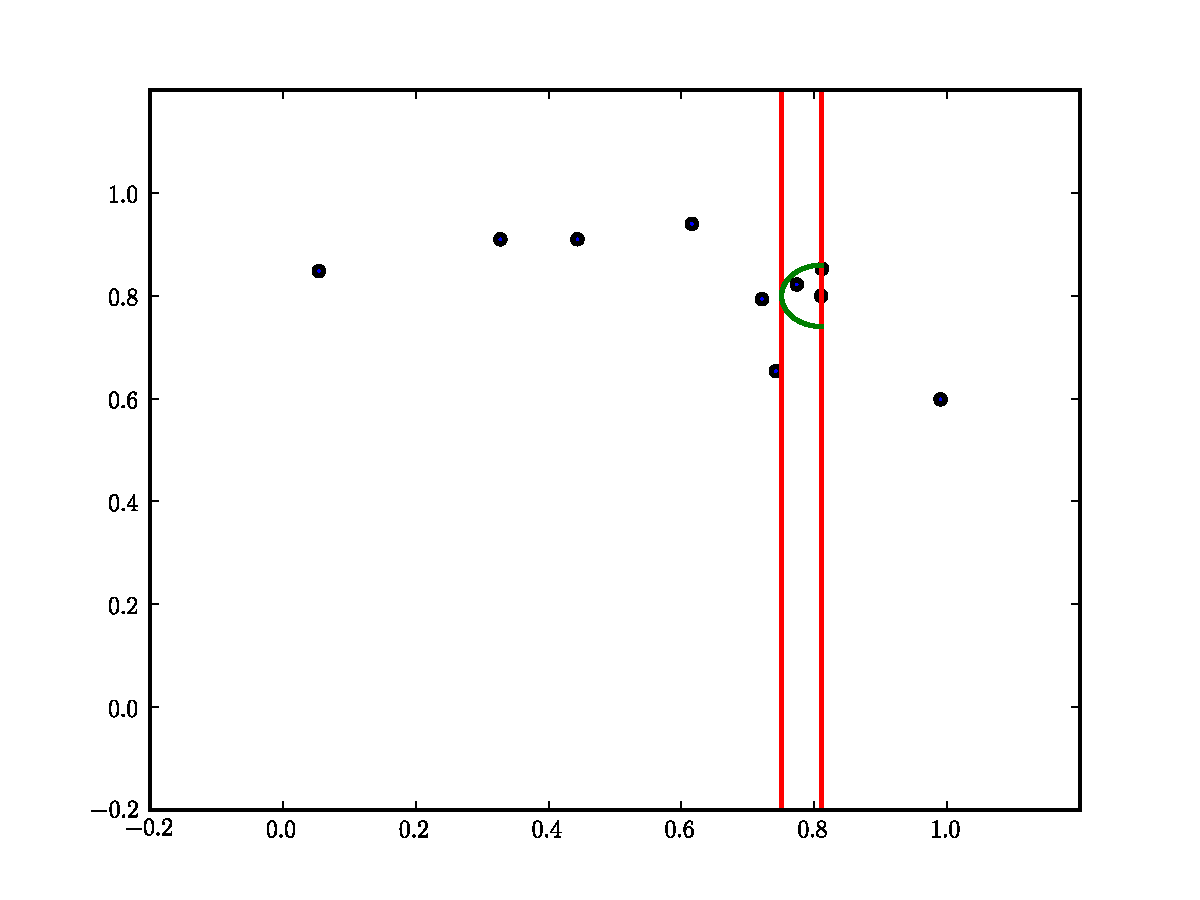
\includegraphics[width = \textwidth]{simple5.pdf}
\caption{A few points further in we actually hit the minimum distance.}
\end{figure}

\begin{figure}[H]
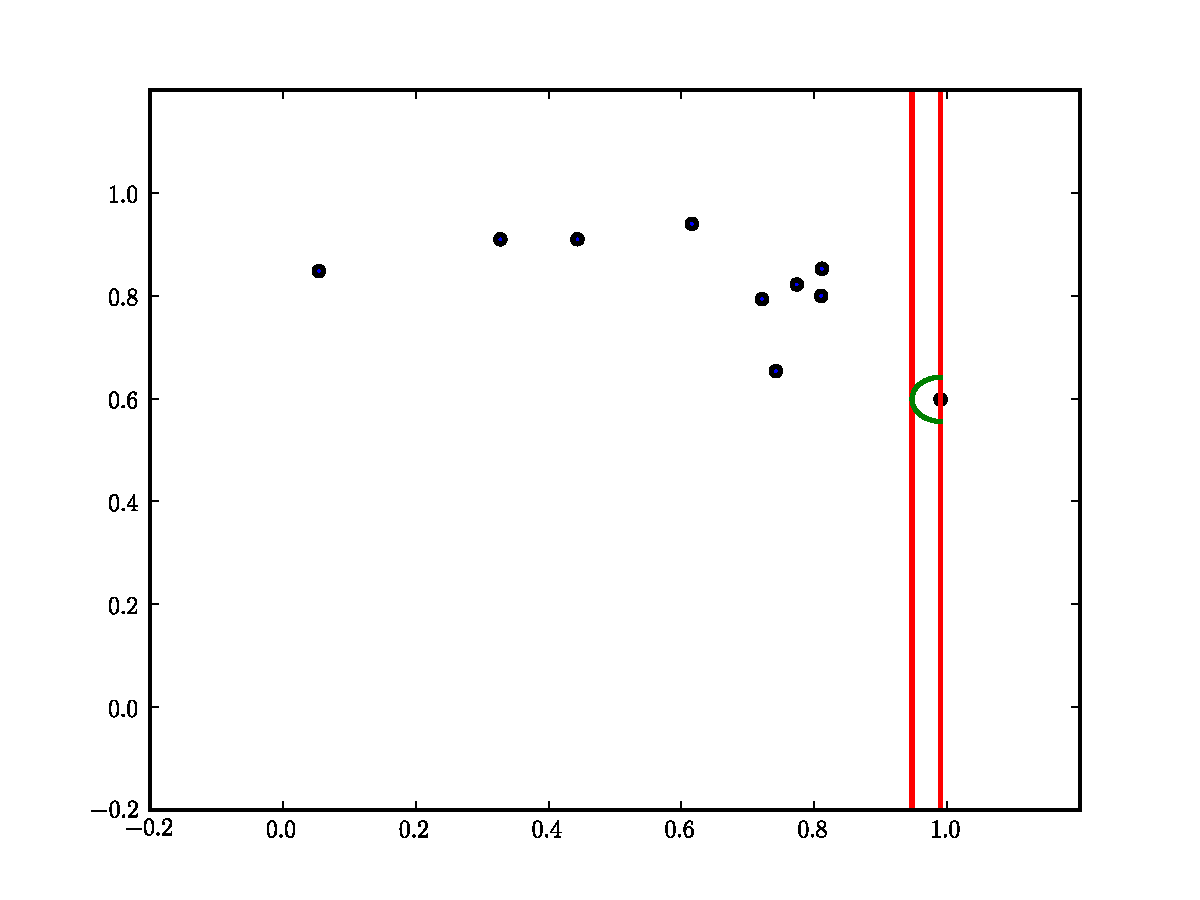
\includegraphics[width = \textwidth]{simple7.pdf}
\caption{After iterating over all the points in the set, we have the final minimum distance desired.}
\end{figure}

\begin{problem}
Write a Python function that implements the above algorithm.
Have your code accept a metric function as a parameter.
This metric function should take a point and an array of points as arguments and return an array of distances from the point to each of the points in the array. 
Test your function's speed. 
How does it scale as you increase the number of points? 
How does it scale as you increase the number of dimensions?
\end{problem}

\section*{A Line Sweep Algorithm}

You may have noticed that we are not exploiting all the symmetry of the problem in the previous algorithm. 
It would likely speed things up if we could also slice away the points that have $y$ values that could not possibly yield the minimum distance. 
The simplest way to do this in this case is to take advantage of some algebraic symmetry.
As we compute the distance between two points, we have to calculate the difference between each of the corrdinates of the points in question. 
If at any time the difference has an absolute value greater than the minimum distance we have encountered thus far, we know we don't need to finish processing the point.
This is, theoretically, like slicing along the other axes in order to further reduce the "active" list of points.
A similar result could be obtained by using a list, binary tree, or some other data structure to keep the list of active points sorted by $y$ value, but in this case the insertion and deletion operations involved are more costly.

This algorithm can be illustrated as follows:

Note: in this case we sweep along the $x$ axis from right to left.

\begin{figure}[H]
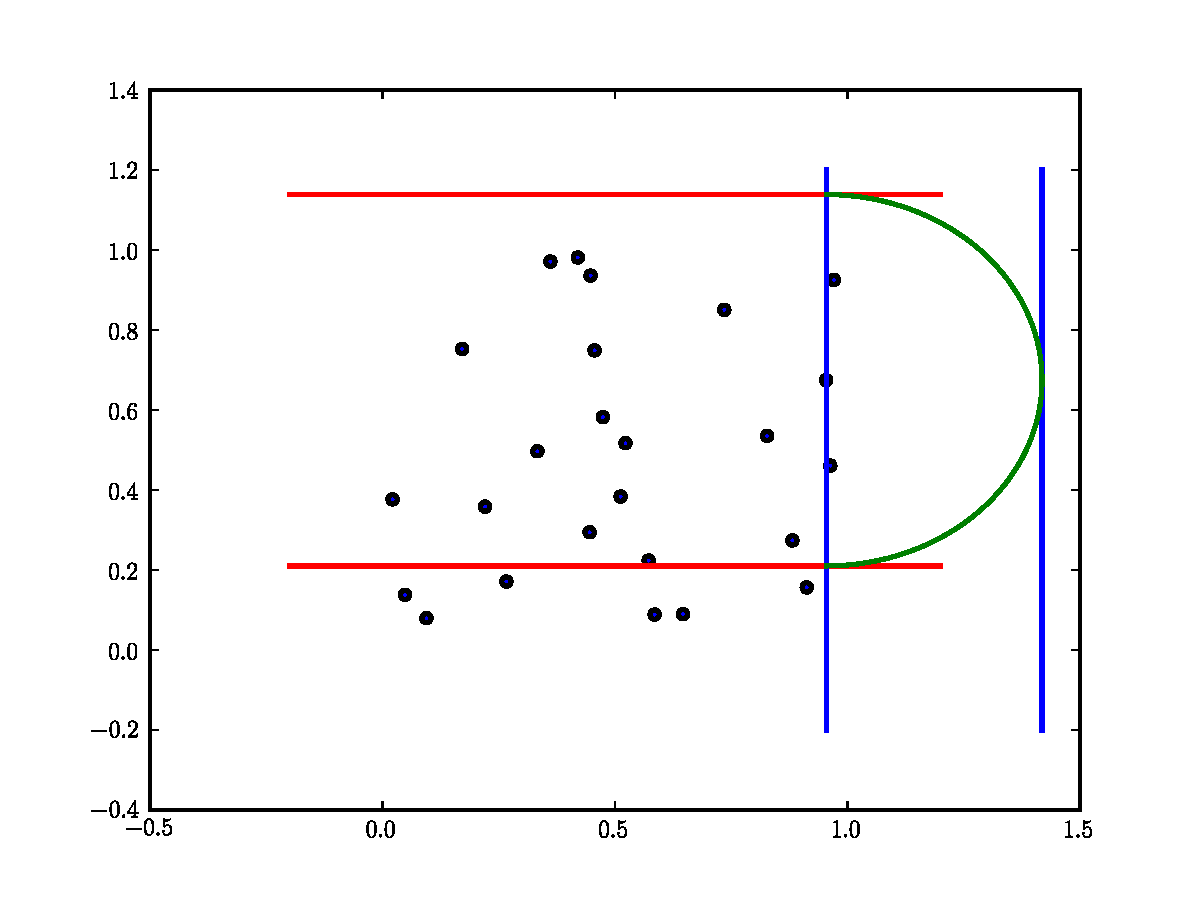
\includegraphics[width = \textwidth]{sweep0.pdf}
\caption{In processing the first point, we find find that we must reduce the radius.
Notice that we only need to consider the points that lie in the box formed by the red an blue lines.}
\end{figure}

\begin{figure}[H]
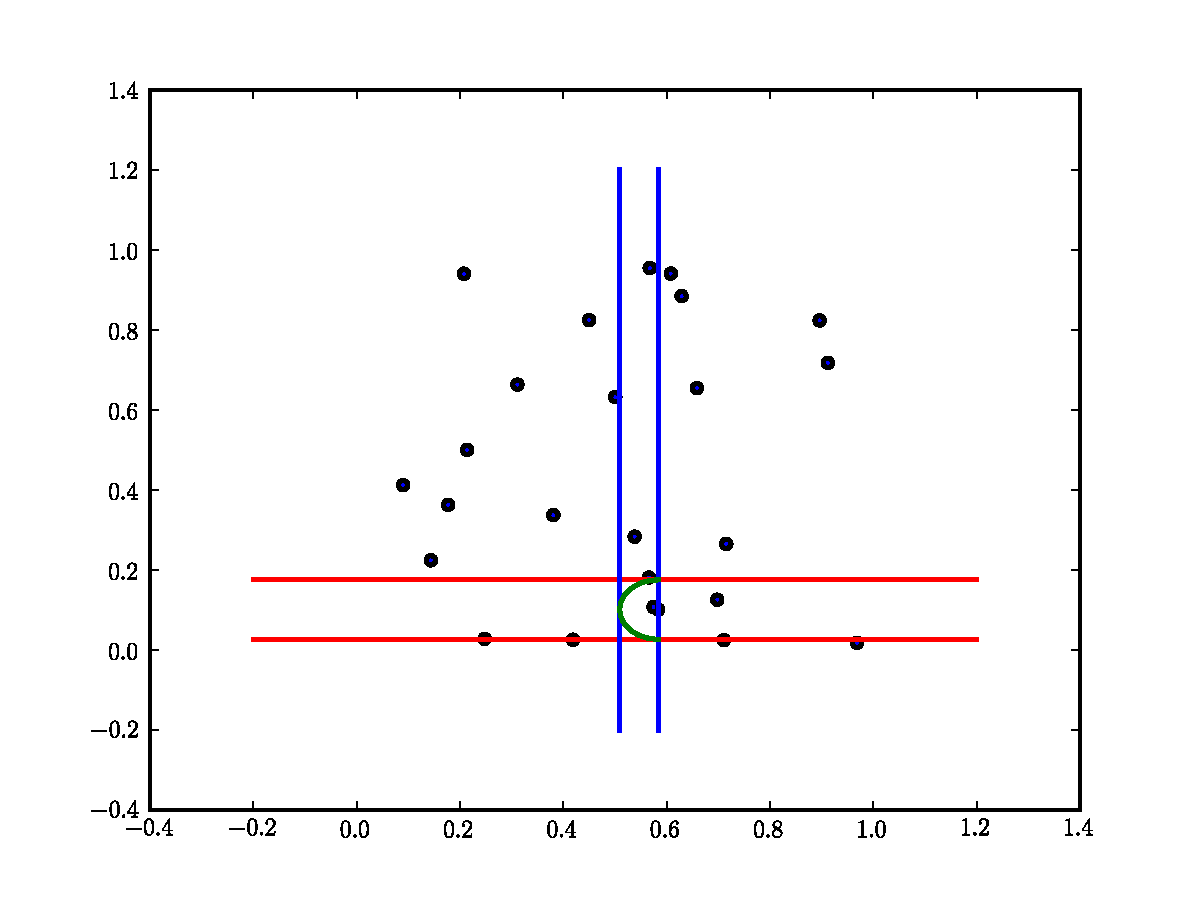
\includegraphics[width = \textwidth]{sweep13.pdf}
\caption{This is where we actually hit the minimum distance.}
\end{figure}

\begin{figure}[H]
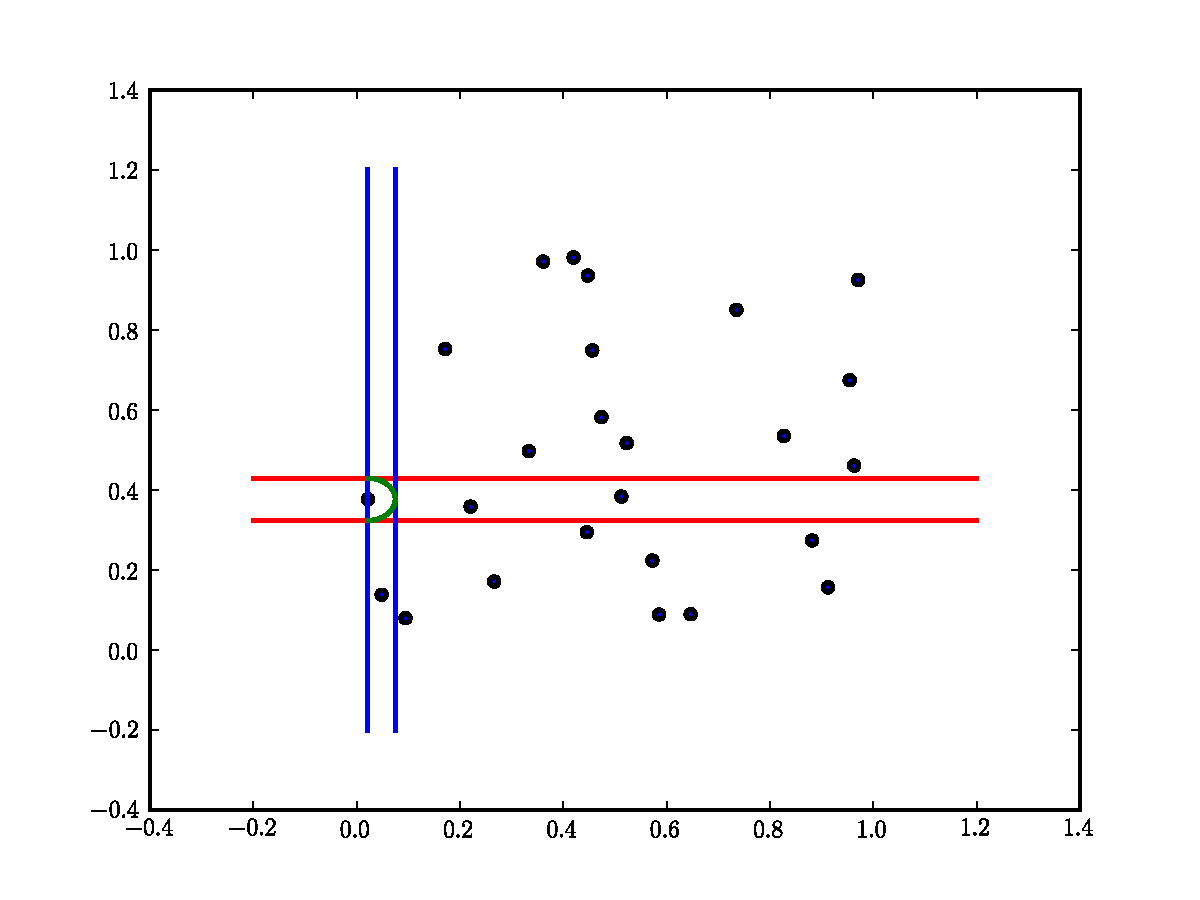
\includegraphics[width = \textwidth]{sweep22.pdf}
\caption{After processing through all the points, we are guaranteed to have hit the minimum distance already, so our minimum distance thus far is our final return value.}
\end{figure}

It is worth noting that this algorithm is based primarily on for loops and array lookups, so it will be much faster if it is written in Cython.
Cython is a Python-based language that allows easy optimization of things like conditional blocks and loops.
We will explain how to use Cython later on in the lab manuals.

\begin{problem}
Implement the algorithm above in Python. 
Time it against the naive implementation at the beginning of this lab and against the simplified version you coded above.
The new version should be faster, but speed depends heavily on how you have implemented it, so you may have some optimization left to do.
Time how long it takes your new function to process ten million points in two dimensions. 
Using benchmarks from the first implementation we gave you, estimate how long (in years) it would take that function to process that many points.
How many times faster is the good implementation?
\end{problem}
